\chapter{Enhanced Super-Resolution Generative Adversarial Network} \label{chap:ESRGAN}

Kolejny omawiany algorytm rozwiązuje problem super-rozdzielczości obrazów przy użyciu Generatywnych Sieci Przestawnych. Algorytm został opracowany przez: Xintao Wang, Ke Yu, Shixiang Wu, Jinjin Gu, Yihao Liu,
Chao Dong, Chen Change Loy, Yu Qiao, Xiaoou Tang \cite{wang2018esrgan}.

\textbf{ESRGAN} jest rozwinięciem algorytmu \textbf{SRGAN} \cite{Ledig_2017_CVPR}; wprowadza kilka istotnych zmian, które znacznie poprawiają jakość obrazów wygenerowanych przez sieć. W tej pracy badane są zalety zastosowanych zmian w architekturze sieci generatora i dyskryminatora, oraz funkcji straty. 


\begin{figure}[ht]
    \centering
    \begin{minipage}[t]{0.4\linewidth}
        
\includegraphics[width=\linewidth]{Rozdziały/02.Podstawy_teoretyczne/Obrazy/comic.png}
        \caption{Obraz wejściowy}
        \label{fig:image60}
    \end{minipage}
    \hspace{0.5cm}
    \begin{minipage}[t]{0.4\linewidth}
        
\includegraphics[width=\linewidth]{Rozdziały/02.Podstawy_teoretyczne/Obrazy/comic_ESRGAN_x4.png}
        \caption{Obraz powiększony algorytmem \textbf{ESRGAN} czterokrotnie}
        \label{fig:image61}
    \end{minipage}
\end{figure}

\newpage
\section{Architektura ESRGAN}

Algorytm \textbf{ESRGAN} bazuje na założeniach \textbf{SRGAN} \cite{Ledig_2017_CVPR}, jednak wprowadza istotne zmiany w architekturze sieci, przeciwnych strat i strat percepcyjnych.

\begin{figure}[ht]
    \centering
    \begin{minipage}[t]{0.85\linewidth}
        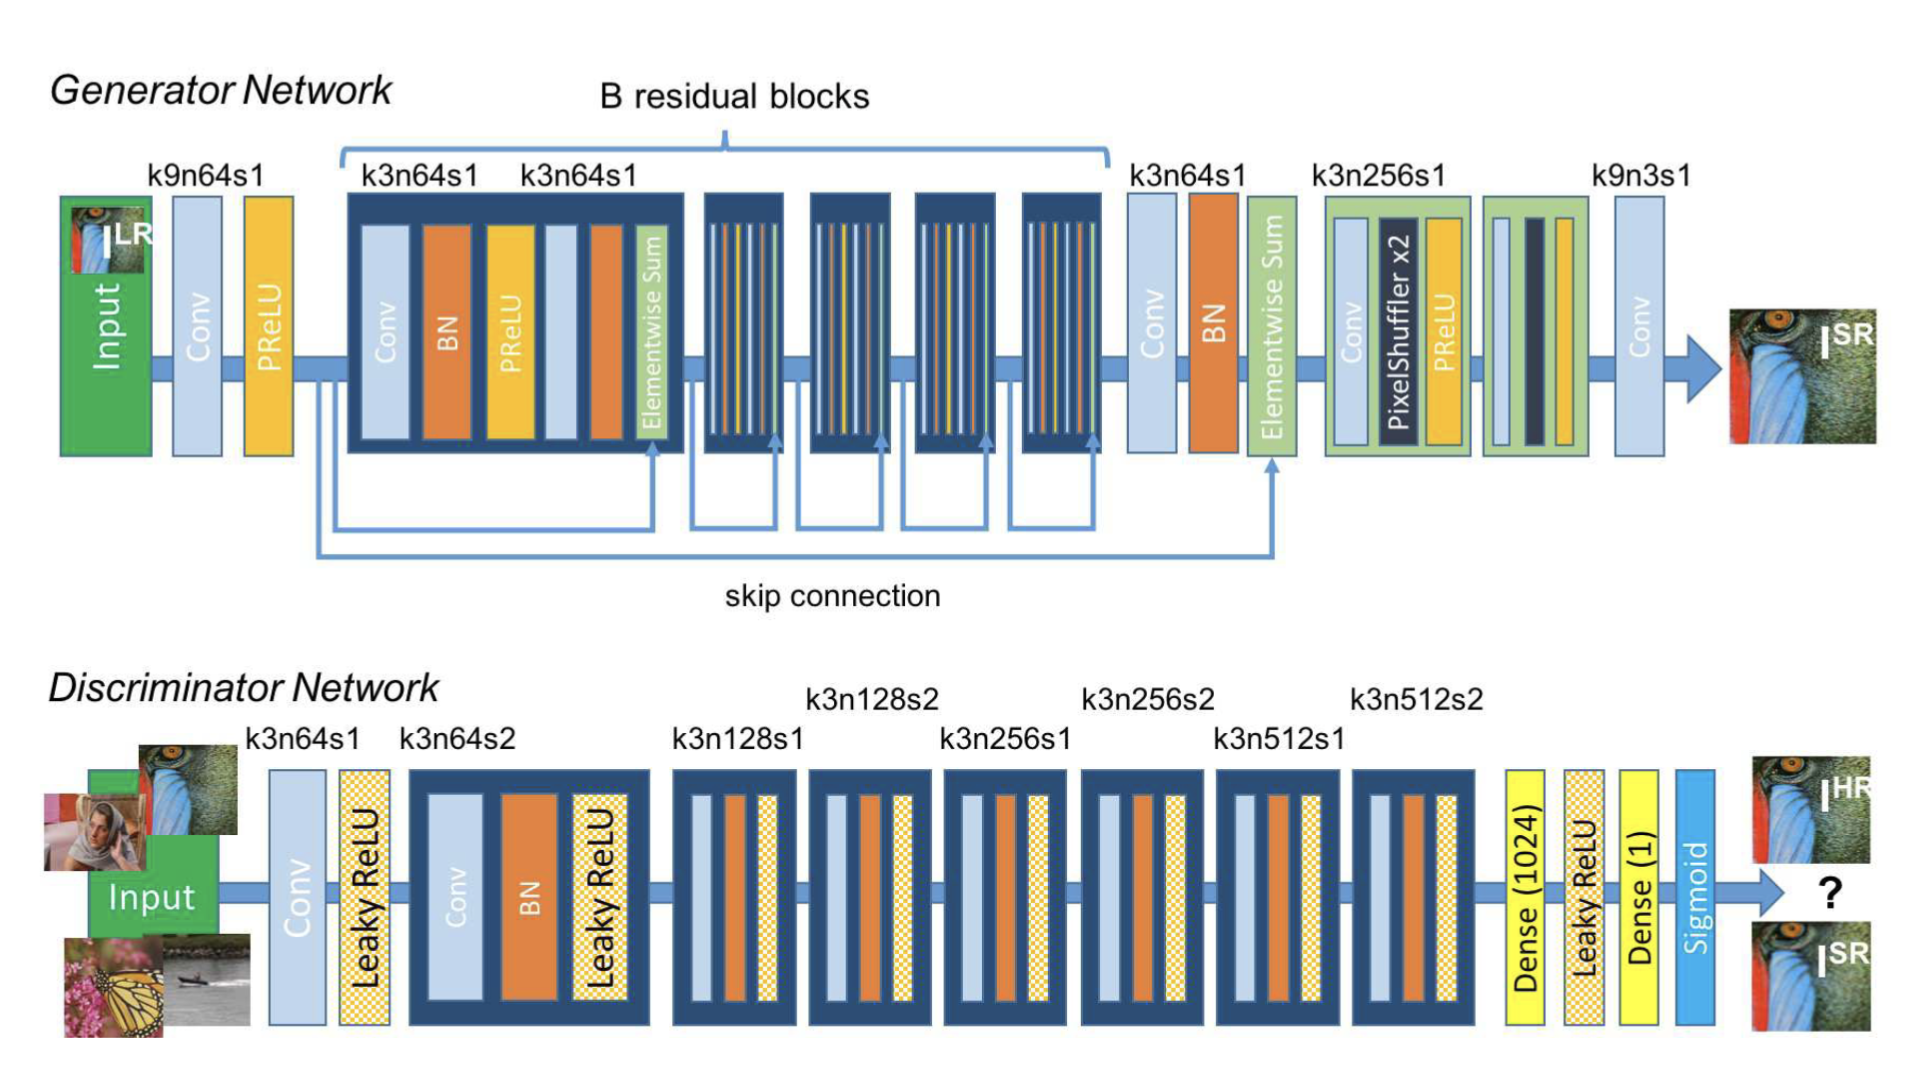
\includegraphics[width=\linewidth]{Rozdziały/04.ESRGAN/Obrazy/Architektura SRGAN.png}
        \caption{Architektura \textbf{SRGAN}}
        \label{fig:image62}
    \end{minipage}
\end{figure}

Architektura \textbf{SRGAN} składa się z dwóch sieci: generatora i dyskryminatora [Rys \ref{fig:image62}]. Generator przyjmuje na wejściu obraz o niskiej rozdzielczości i zwraca obraz o wysokiej rozdzielczości. Dyskryminator przyjmuje na wejściu obraz o wysokiej rozdzielczości i zwraca prawdopodobieństwo, że obraz jest rzeczywisty, a nie wygenerowany przez sieć. 

\textbf{SRGAN} wykorzystuje VGG loss, czyli funkcję straty opartą na głębokiej sieci neuronowej VGG, używaną do oceny podobieństwa percepcyjnego między obrazami. Zamiast mierzyć różnicę pomiędzy pikselami, jak w przypadku błędu średniokwadratowego (MSE), VGG loss porównuje cechy reprezentacyjne (np. tekstury, kształty) wyekstrahowane przez sieć VGG z obu obrazów. Poprzez użycie tej funkcji straty, SRGAN skupia się na generowaniu obrazów, które są percepcyjnie bardziej podobne do obrazów wysokiej rozdzielczości, zamiast jedynie minimalizować błąd średniokwadratowy. Dzięki temu, generowane obrazy charakteryzują się lepszą jakością percepcyjną, bardziej zbliżoną do naturalnych zdjęć.



\textbf{ESRGAN} wprowadza kilka istotnych zmian w architekturze sieci. Zmiany te mają na celu poprawę jakości generowanych obrazów i eliminację artefaktów na obrazach wyjściowych.


\subsection*{Zmiany w architekturze}

\begin{figure}[ht]
    \centering
    \begin{minipage}[t]{0.85\linewidth}
        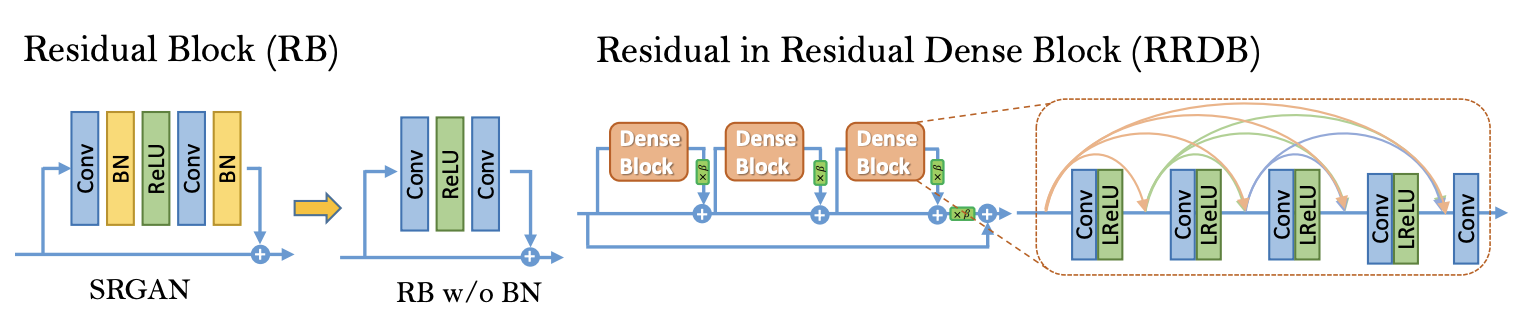
\includegraphics[width=\linewidth]{Rozdziały/04.ESRGAN/Obrazy/Architektura ESRGAN 1.png}
        \caption{Zmiany zastosowane w architekturze \textbf{ESRGAN}}
        \label{fig:image63}
    \end{minipage}
\end{figure}

Pierwszą zmianą było usunięcie warstw normalizacji wsadowej z generatora (lewa strona Rys \ref{fig:image63}). 
Normalizacja wsadowa jest techniką stosowaną w procesie uczenia sieci neuronowych, która ma na celu poprawę stabilności i szybkości uczenia poprzez normalizację danych wejściowych w każdej warstwie na podstawie mini-zestawów (batchy). Technika ta polega na dostosowaniu średniej i wariancji danych w każdym mini-zestawie, co pomaga w redukcji problemu zwanego "wewnętrznym przesunięciem kowariancji" (internal covariance shift) i sprzyja szybszemu i bardziej stabilnemu uczeniu sieci.

Warstwy te powodowały, że obrazy wyjściowe posiadały artefakty [Rys \ref{fig:image64}] - powtarzające się tekstury.

\begin{figure}[ht]
    \centering
    \begin{minipage}[t]{0.85\linewidth}
        \includegraphics[width=\linewidth]{Rozdziały/04.ESRGAN/Obrazy/Batch normalization artefacts.png}
        \caption{Przykłady artefaktów powstałych przez normalizację wsadową}
        \label{fig:image64}
    \end{minipage}
\end{figure}

Kolejną zmianą było powiększenie ilości warstw w generatorze (prawa strona Rys \ref{fig:image63}). W \textbf{SRGAN} generator składał się z 16 warstw, natomiast w \textbf{ESRGAN} z 23 warstw. Zwiększenie ilości warstw pozwoliło na zwiększenie złożoności sieci, co przełożyło się na lepszą jakość generowanych obrazów.

\subsection*{Zmiany w dyskryminatorze}

W \textbf{ESRGAN} zastosowano zmiany nie tylko w generatorze, ale również w dyskryminatorze stosując dyskryminator relatywistyczny \cite{jolicoeurmartineau2018relativistic}. Dyskryminator stosowany w \textbf{SRGAN} zwracał prawdopodobieństwo, że obraz jest rzeczywisty, a nie wygenerowany przez sieć. Dyskryminator relatywistyczny przewiduje prawdopodobieństwo czy obraz prawdziwy jest relatywnie bardziej realistyczny niż obraz wygenerowany przez generator [Rys \ref{fig:image66}].

\begin{figure}[ht]
    \centering
    \begin{minipage}[t]{0.85\linewidth}
        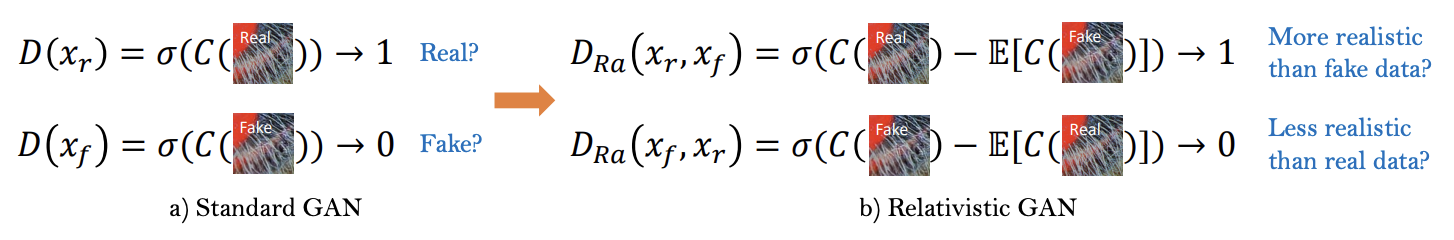
\includegraphics[width=\linewidth]{Rozdziały/04.ESRGAN/Obrazy/relatywistyczny dyskryminator.png}
        \caption{Różnica między dyskryminatorem standardowym a relatywistycznym}
        \label{fig:image66}
    \end{minipage}
\end{figure}

\subsection*{Zmiany w funkcji straty}

Zastosowano również zmianę w funkcji straty. Zastosowano funkcję strat VGG, ale mapy cech były porównywane przed aktywacją, a nie po. Porównanie cech przed aktywacją pozwala wykorzystanie większej ilości informacji, gdyż mapy aktywacji są gęstsze i zawierają więcej informacji o obrazie przed analizą przez funkcję aktywacji [Rys \ref{fig:image65}].

\begin{figure}[ht]
    \centering
    \begin{minipage}[t]{0.85\linewidth}
        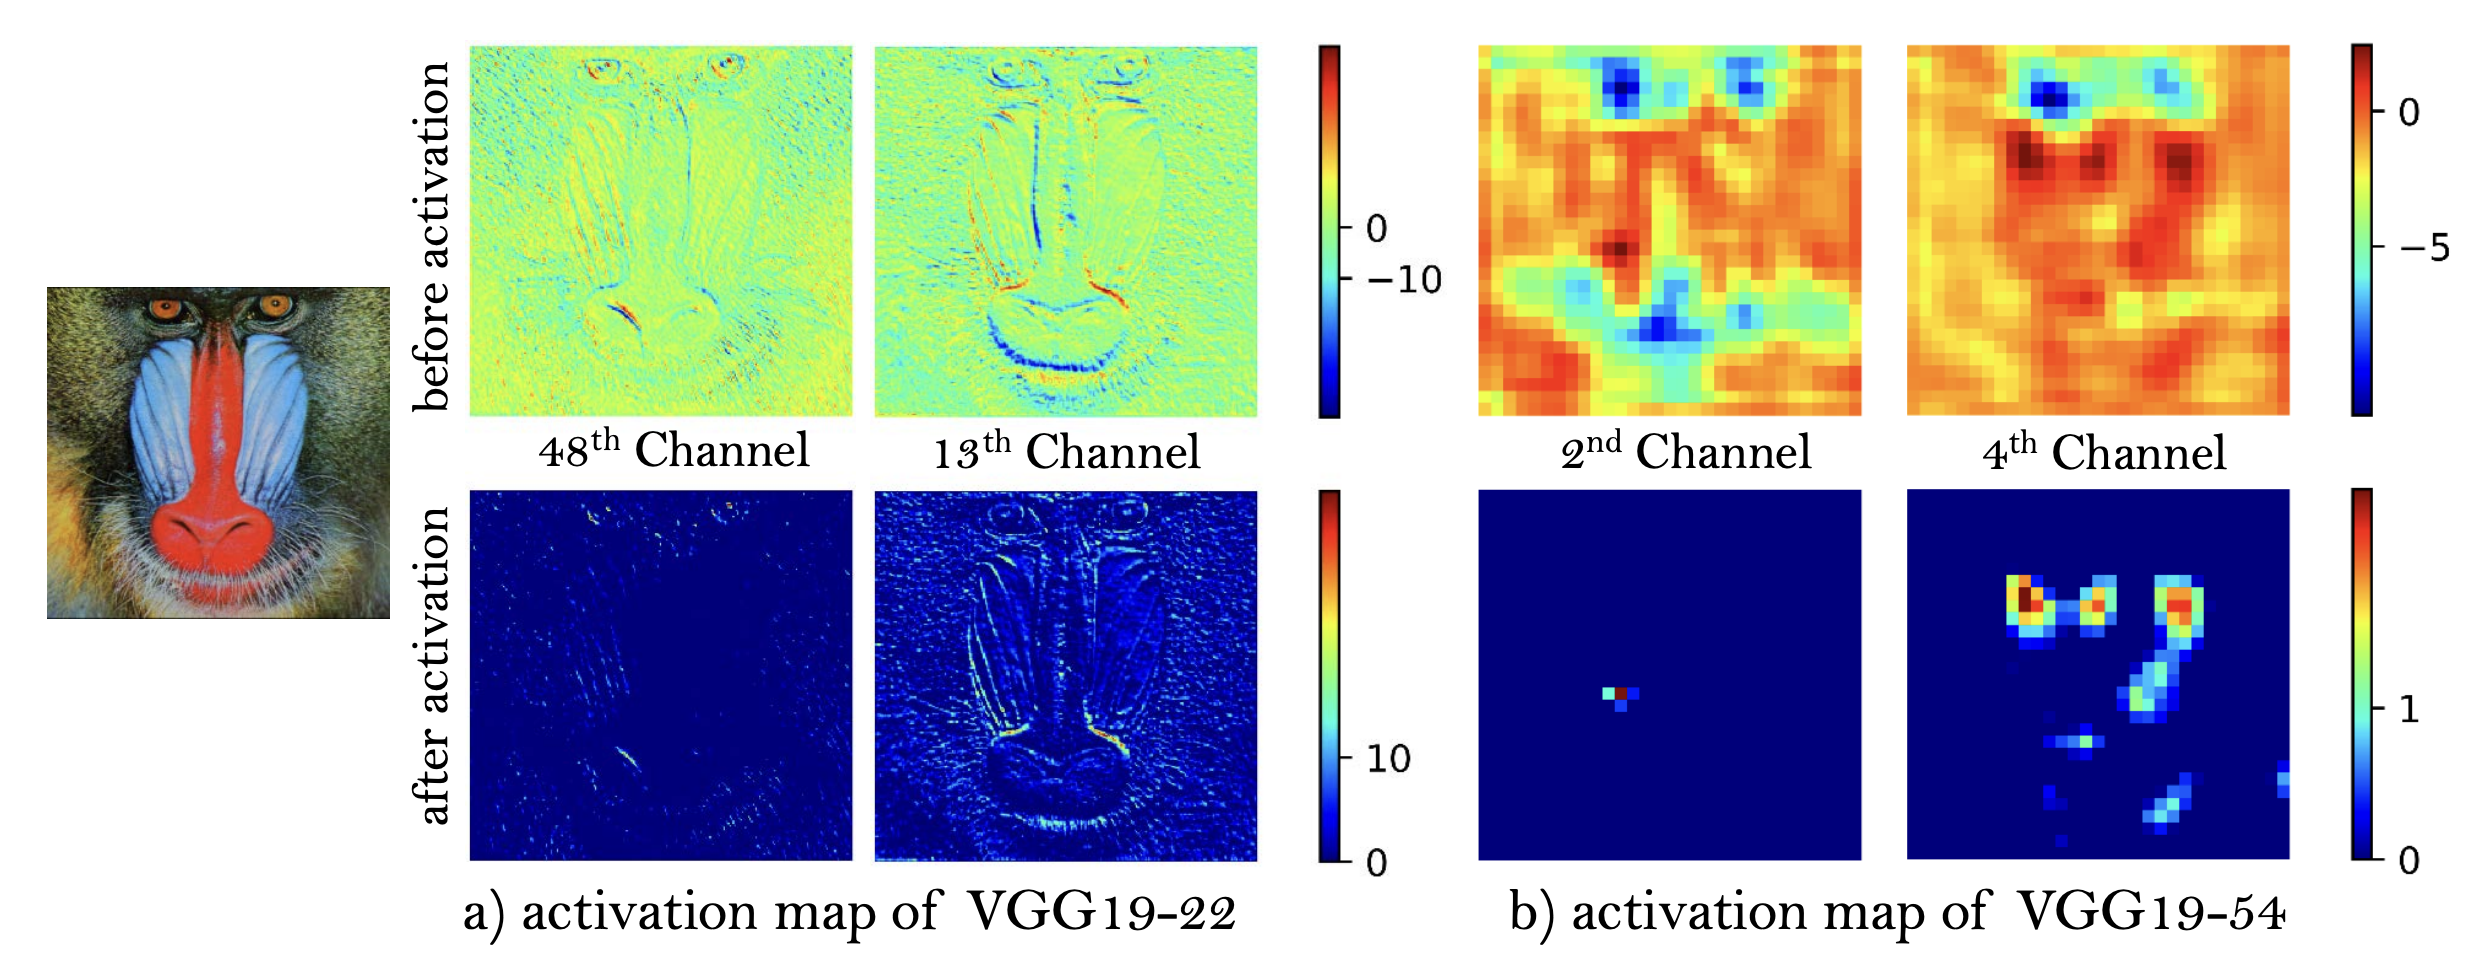
\includegraphics[width=\linewidth]{Rozdziały/04.ESRGAN/Obrazy/mapa aktywacji.png}
        \caption{Mapa cech przed aktywacją i po aktywacji}
        \label{fig:image65}
    \end{minipage}
\end{figure}



\section{Proces treningu}

Podobnie jak w \textbf{SRGAN} \cite{Ledig_2017_CVPR}, w \textbf{ESRGAN} \cite{wang2018esrgan} obrazy powiększane są ze skalą 4 pomiędzy obrazami $LR$ a $HR$. 

Do treningu \textbf{ESRGAN} wykorzystano bazę danych DIV2K \cite{Agustsson_2017_CVPR_Workshops}, która zawiera 800 zdjęć o wysokiej rozdzielczości (2k), oraz zbioru danych Flickr2K % \cite{lim2017enhanced}
, który zawiera 2650 zdjęć o takiej samej rozdzielczości. Dodatkowo wzbogacono zestaw treningowy o losowe odbicia lustrzane i rotacje o 90 stopni.


Obrazy $HR$ przeskalowano z użyciem Matlaba. Używano mini-zestawów (mini-batch) o wielkości 16 i kadrowano fragmenty HR o rozmiarze $128 \times 128$ pikseli. Większy rozmiar fragmentów pomagał w przechwytywaniu większej ilości informacji semantycznej, co było korzystne dla głębszych sieci, ale zwiększało czas treningu i zapotrzebowanie na zasoby obliczeniowe.

Do optymalizacji użyto metody Adam z parametrami \( \beta_1 = 0.9 \) i \( \beta_2 = 0.999 \), aktualizując na przemian sieci generatora i dyskryminatora do momentu zbieżności modelu.

Jako zestaw testowy wykorzystano obrazy z zestawów danych Set5 \cite{bevilacqua2012low}, Set14 \cite{zeyde2010single}, BSD100 \cite{martin2001database} i Urban100 \cite{Huang_2015_CVPR}.



\section{Przykłady zastosowań i rezultaty}

Przykładowe wyniki działania algorytmu \textbf{ESRGAN} przedstawiono na Rys: \ref{fig:image68} \ref{fig:image70}, \ref{fig:image72}. Obrazy pochodzą z repozytorium GitHub, gdzie umieszczony został również algorytm \textbf{DWSR} \cite{guo2017deep}.

Omawiany algorytm radzi sobie jeszcze lepiej niż opisywany w poprzednim rozdziale \textbf{DWSR}, zwłaszcza z teksturami takimi jak włosy, czy futro. \textbf{ESRGAN} świetnie radzi sobie z krawędziami obiektów na obrazach, widać to na przykładzie Rys. \ref{fig:image70}, gdzie ramy okien są bardzo wyraźnie zarysowane.

Jako, że \textbf{ESRGAN} jest dużym i skomplikowanym modelem jego czas egzekucji jest znacznie dłuższy niż w przypadku \textbf{DWSR}. 

Dokładniejsza analiza działania algorytmu \textbf{ESRGAN}, oraz analiza porównawcza z algorytmem \textbf{DWSR} została przedstawiona w Rozdziale \ref{chap:porownanie_algorytmow}.


\begin{figure}[ht]
    \centering
    \begin{minipage}[t]{0.45\linewidth}
        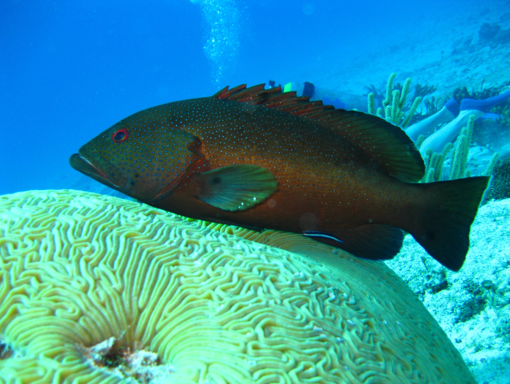
\includegraphics[width=\linewidth]{Rozdziały/03.DWSR/Obrazy/0904x4.png}
        \caption{Obraz wejściowy}
        \label{fig:image67}
    \end{minipage}
    \hspace{0.5cm}
    \begin{minipage}[t]{0.45\linewidth}
        \includegraphics[width=\linewidth]{Rozdziały/03.DWSR/Obrazy/0904x4_ESRGANx4.png}
        \caption{Obraz powiększony algorytmem \textbf{ESRGAN} czterokrotnie}
        \label{fig:image68}
    \end{minipage}
\end{figure}

\begin{figure}[ht]
    \centering
    \begin{minipage}[t]{0.45\linewidth}
        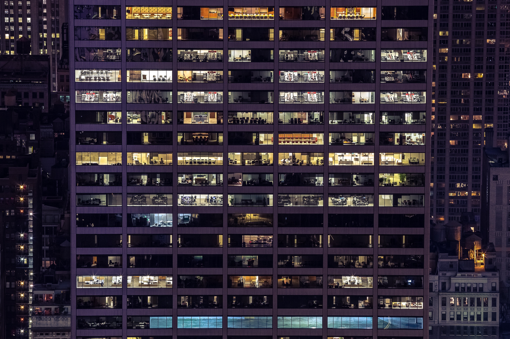
\includegraphics[width=\linewidth]{Rozdziały/03.DWSR/Obrazy/0913x4.png}
        \caption{Obraz wejściowy}
        \label{fig:image69}
    \end{minipage}
    \hspace{0.5cm}
    \begin{minipage}[t]{0.45\linewidth}
        \includegraphics[width=\linewidth]{Rozdziały/03.DWSR/Obrazy/0913x4_ESRGANx4.png}
        \caption{Obraz powiększony algorytmem \textbf{ESRGAN} czterokrotnie}
        \label{fig:image70}
    \end{minipage}
\end{figure}

\begin{figure}[ht]
    \centering
    \begin{minipage}[t]{0.45\linewidth}
        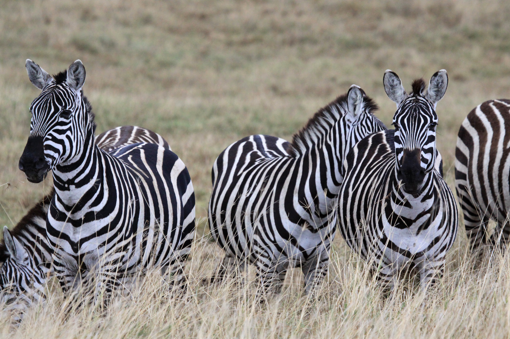
\includegraphics[width=\linewidth]{Rozdziały/03.DWSR/Obrazy/0999x4.png}
        \caption{Obraz wejściowy}
        \label{fig:image71}
    \end{minipage}
    \hspace{0.5cm}
    \begin{minipage}[t]{0.45\linewidth}
        \includegraphics[width=\linewidth]{Rozdziały/03.DWSR/Obrazy/0999x4_ESRGANx4.png}
        \caption{Obraz powiększony algorytmem \textbf{ESRGAN} czterokrotnie}
        \label{fig:image72}
    \end{minipage}
\end{figure}